\documentclass{article}
\usepackage{amsmath}
\usepackage{setspace}
\usepackage{tasks}
\usepackage{graphicx}
\usepackage{caption}

\title{Plaformio}
\author{SHAIK MOHAMMAD SAHIL}
\date{OCTOBER 2023}

\begin{document}

\maketitle

\begin{enumerate}
\item In the circuit shown below, P and Q are the inputs. The logical function realized by the circuit shown below

\begin{figure}[h]
\centering
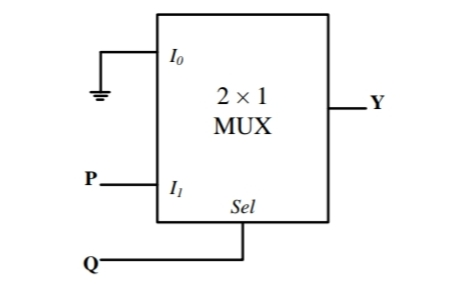
\includegraphics[width=\columnwidth]{/sdcard/platformio/figs/mux.jpg}
\caption{Neglecting the delays}
\label{fig:mux.jpg}
\end{figure}

\hfill(GATE EC 2023)

\begin{enumerate}
    \item Y=PQ
    \item Y=P+Q    
    \item Y= $\overline{PQ}$
    \item Y= $\overline{P+Q}$
\end{enumerate}

\end{enumerate}

\end{document}
